\scanpage{6}
on n'a pas défini pour l'instant de métrique riemannienne intrinsèque intéressante, mais bien des métriques finslériennes. On espère trouver une métrique riemannienne à \uline{courbure négative}, qui permettrait alors par un argument géométrique simple (en utilisant \inserted{l'existence et} l'unicité de la géodésique qui joint deux pts) de prouver que tt gpe fini d'autom. complexes de $\mathcal M_{g,\nu}$ admet un pt fixe. Deligne pense que c'est vrai que tt sous gpe fini de $\Gamma_{g,\nu}$ a un pt fixe dans $\mathcal M_{g,\nu}$, et il ne voit que cette voie d'approche plausible.

\figure{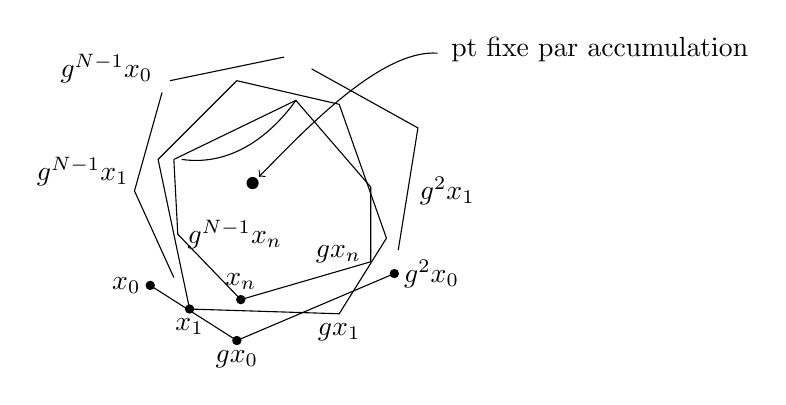
\begin{tikzpicture}[x=1cm,y=1cm]
\draw (-1.6,-.8)--(-.5,-1.5)--(1.5,-.65);
\draw (-1.3,-.7)--(-1.8,.4)--(-1.45,1.65);
\draw (-1.35,1.8)--(.1,2.1);
\draw (.45,1.95)--(1.8,1.2)--(1.55,-.35);
\draw (-1.1,-1.1)--(.8,-1.16)--(1.4,-.2)--(.8,1.5)--(-.5,1.8)--(-1.5,.8)--(-1.1,-1.1);
\draw (-1.3,.8)--(.25,1.55)--(1.2,.45)--(1.2,-.5)--(-.45,-.98)--(-1.25,-.15)--(-1.3,.8);
\draw (-1.2,.8)..controls (-.5,.7) and (0,1.2)..(.25,1.55);
\fill (-1.6,-.8) circle(1.7pt) (-1.1,-1.1) circle(1.7pt) (-.5,-1.5) circle(1.7pt) (1.5,-.65) circle(1.7pt) (-.45,-.98) circle(1.7pt) (-.3,.5) circle(2.2pt);
\node[left] at (-1.6,-.8) {$x_0$};\node[below] at (-1.1,-1.1) {$x_1$};
\node[below] at (-.5,-1.5) {$gx_0$};\node[below] at (.8,-1.16) {$gx_1$};
\node[right] at (1.5,-.65) {$g^2x_0$};\node[right] at (1.7,.4) {$g^2x_1$};
\node[left] at (-1.45,1.95) {$g^{\unsure{N-1}}x_0$};
\node[left] at (-1.75,.65) {$g^{\unsure{N-1}}x_1$};
\node[above] at (-.45,-.98) {$x_n$};\node[left] at (1.2,-.4) {$gx_n$};
\node[right] at (-1.25,-.15) {$g^{\unsure{N-1}}x_n$};
\node[right] at (2.1,2.2) {pt fixe par accumulation};
\draw[->] (2.05,2.15)..controls (1.3,2.2) and (.3,1.1)..(-.22,.58);
\end{tikzpicture}}

8) Mumford connaîtrait la présentation des $\Gamma_{g,\nu}$ (via les générateurs habituels).

L. Bers (Columbia.) ferait de la ``chirurgie complexe'' des surfaces de Riemann pour \deleted{\unsure{définir}} étudier la compactification des $M_{g,\nu}$.

\mspage{5}
